\subsection{Методологія кількісного тестування якості масштабування}

Для забезпечення об'єктивності аналізу та здійснення коректного порівняння якості масштабування розробленого методу з класичними аналогами було застосовано загальноприйняту методологію кількісної оцінки. Оскільки в більшості стандартних тестових датасетів оригінальні вхідні дані для довільних коефіцієнтів масштабування відсутні, формування вибірок для тестування виконується за схемою інверсного моделювання.

Нехай маємо оригінальне зображення $I^{res}$ розміром $n \times m$ з обраного датасету, яке приймається за еталонне. Щоб перевірити якість роботи алгоритмів для довільного коефіцієнта масштабування $s$, генерується спільне для всіх методів вхідне зображення $I^{in}$. Воно створюється шляхом застосування стандартної бікубічної інтерполяції (BIC) до еталону, але у протилежному напрямку масштабування.

На практиці цей процес поділяється на два сценарії, залежно від того, тестується збільшення чи зменшення зображення:
\begin{enumerate}
	\item \textbf{Тестування методів збільшення [$\times s$]:} для оцінки алгоритму вхідна матриця $I^{in}$ генерується шляхом зменшення еталонного зображення $I^{res}$ у $s$ разів за допомогою бікубічної інтерполяції [$: s$]. Після цього будь-який з обраних для тестування методів застосовується до цього низькороздільного кадру $I^{in}$, а отриманий результат порівнюється з початковим еталоном $I^{res}$.
	
	\item \textbf{Тестування методів зменшення (Downscaling [$: s$]):} для оцінки алгоритму стиснення вхідне зображення $I^{in}$ формується шляхом збільшення еталону $I^{res}$ у $s$ разів [$\times s$]. Потім результат роботи досліджуваного методу, застосованого до $I^{in}$, порівнюється з первинним еталоном $I^{res}$.
\end{enumerate}

Такий підхід дозволяє нівелювати вплив сторонніх чинників і забезпечує абсолютно рівні початкові умови для тестування як розробленого алгоритму, так і індустріальних стандартів. Наочно схема процесу тестування зображена на рисунку~\ref{fig:test_scheme}.

\begin{figure}[htbp]
	\centering
	% Увага: заміни 'testing_scheme.png' на точну назву свого файлу зі схемою
	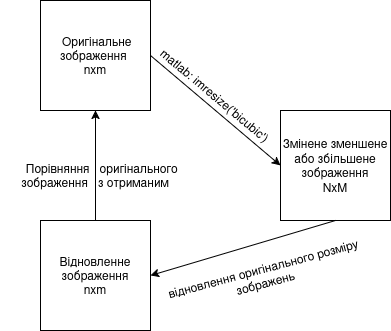
\includegraphics[width=0.8\textwidth]{figures/TestDiagram.drawio.png}
	\caption{Схема генерації тестових вибірок та порівняння результатів}
	\label{fig:test_scheme}
\end{figure}

Такий підхід гарантує прозорість експерименту та дозволяє на основі кількісних метрик об'єктивно оцінити ефективність розробленого алгоритму та порівняти його з індустріальними стандартами.